\documentclass[a4paper, 12pt]{article}

\usepackage{fontspec}
\usepackage{polyglossia}
\defaultfontfeatures{Ligatures=TeX}
\setdefaultlanguage{russian}
\setotherlanguage{english}
\setmainfont{Times New Roman}
\newfontfamily{\latinfont}{Times New Roman}
\newfontfamily{\cyrillicfont}{Times New Roman}
\newfontfamily{\cyrillicfonttt}{Courier New}

\usepackage{geometry}
\usepackage{amsmath}
\usepackage{amssymb}
\usepackage{amsfonts}
\usepackage{graphicx}
\usepackage{float}
\usepackage{wrapfig}
\usepackage{subcaption}
%\usepackage[caption=false]{subfig}
\geometry{right=20mm}
\geometry{left=20mm}
\geometry{top=20mm}
\geometry{bottom=20mm}

\usepackage{indentfirst}
\usepackage[outputdir=auxiliary]{minted}

\graphicspath{{../img/}}
\DeclareMathOperator{\R}{\mathbb{R}}
\DeclareMathOperator{\C}{\mathbb{C}}
\renewcommand{\Re}{\mathrm{Re}}
\renewcommand{\Im}{\mathrm{Im}}


\begin{document}
    \begin{titlepage}
    \begin{center}
        \textit{МИНИСТЕРСТВО ОБРАЗОВАНИЯ И НАУКИ\\
        РОССИЙСКОЙ ФЕДЕРАЦИИ}
        \vspace{1ex}

        федеральное государственное бюджетное образовательное учреждение\\
        высшего профессионального образования
        \vspace{1ex}

        \textbf{САНКТ-ПЕТЕРБУРГСКИЙ НАЦИОНАЛЬНЫЙ ИССЛЕДОВАТЕЛЬСКИЙ УНИВЕРСИТЕТ ИТМО}
        \vspace{13ex}

        Лабораторная работа №3\\
        <<Динамика нелинейных систем>>\\
        по дисциплине <<Моделирование технических систем>>\\
        \vspace{1em}
        Вариант 3\\
    \end{center}
    \vspace{14em}
    \begin{flushright}
        \noindent
        Выполнили:\\
        студенты гр. R4133c\\
        Борисов М. В.\\
        Симонов П.\\
        Мацуганов А. И.\\
        \vspace{1em}
        Преподаватель:\\
        Семенов Д. М.
    \end{flushright}
    \vfill
    \begin{center}
        \large{Санкт-Петербург}\\
        2021 г.\\
    \end{center}
\end{titlepage}

    \setcounter{page}{2}
    \setlength{\parindent}{0pt}

    \section*{Задание 1}
    Дана нелинейная система.
    \begin{equation*}
        \left\{
        \begin{aligned}
            \dot{x} &= -3x + y\\
            \dot{y} &= x - 4y - \arctan{2y}
        \end{aligned}
        \right.
    \end{equation*}

    \begin{enumerate}
        \item Найти её положения равновесия
        \item Линеаризовать систему около одного из положений равновесия, исследовать на устойчивость
        \item Доказать устойчивость исходной системы с помощью метода функций Ляпунова
        \item Построить графики исходной и линеаризованной систем
    \end{enumerate}

    \subsection*{Решение}
    \subsubsection*{Найдём положение равновесия}
    \begin{equation*}
        \left\{
        \begin{aligned}
            &-3x_1 + x_2 = 0 \\
            &x_1 - 4x_2 - \arctan{2x_2} = 0
        \end{aligned}
        \right.
    \end{equation*}
    \begin{equation*}
        \left\{
        \begin{aligned}
            &x_2 = 3x_1 \\
            &11x_1 = -\arctan{6x_1}
        \end{aligned}
        \right.
    \end{equation*}

    \[x^* = (0,\,0)\]

    \subsubsection*{Исследуем на устойчивость около положения равновесия}
    \begin{equation*}
        A(x) =
        \begin{bmatrix}
            -3& 1\\
            1& -\dfrac{6 + 16x^2}{1 + 4x^2}
        \end{bmatrix}
    \end{equation*}

    \begin{equation*}
        A(x^*) =
        \begin{bmatrix}
            -3& 1\\
            1& -6
        \end{bmatrix}
    \end{equation*}

    Собственные числа матрицы $A(x^*)$

    \begin{equation*}
        \begin{aligned}
            \lambda_1 &= -6.30 \\
            \lambda_2 &= -2.70
        \end{aligned}
    \end{equation*}

    Оба числа действительные и отрицательные, значит система устойчива и имеет положение равновесия типа "узел".

    \begin{figure}[H]
        \centering
        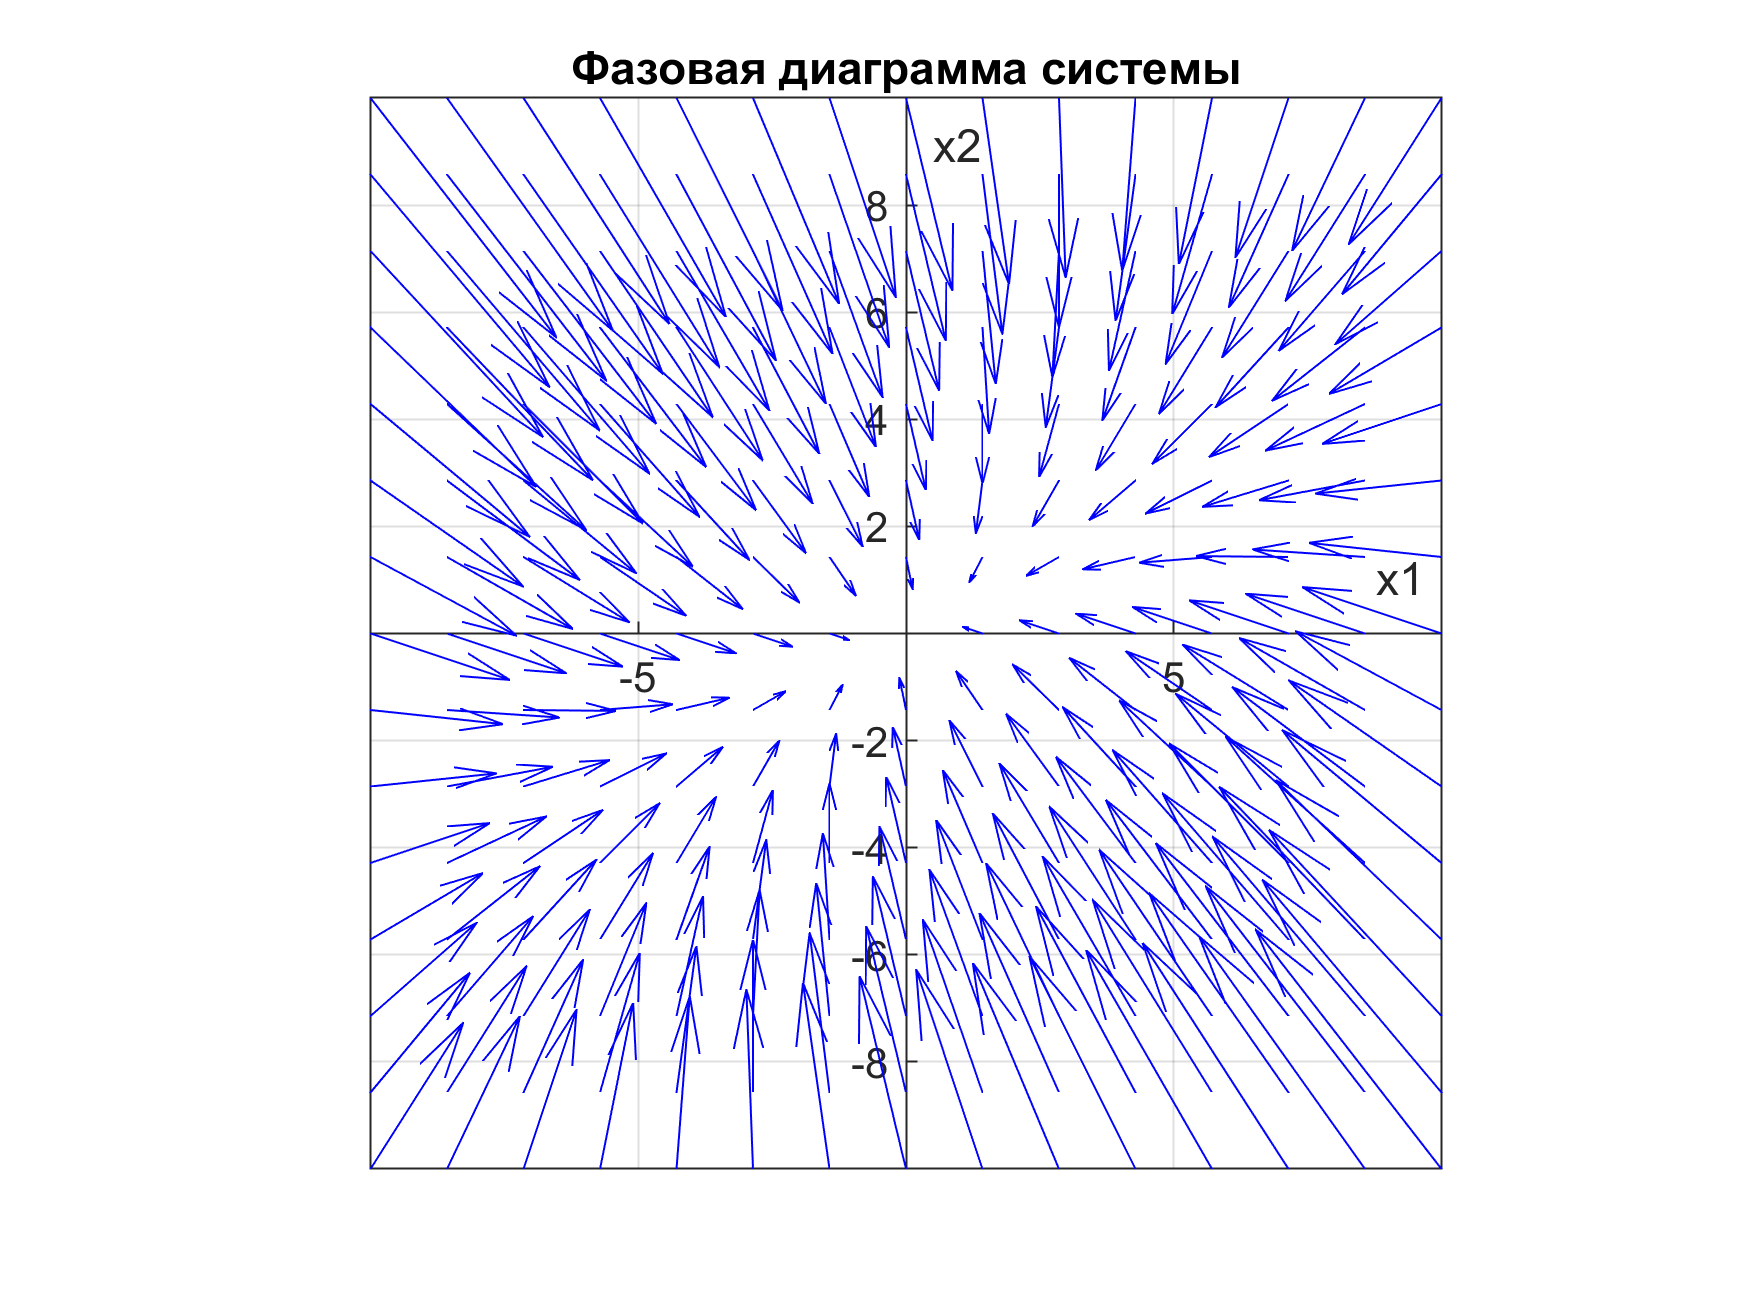
\includegraphics[width=0.7\textwidth]{phase.png}
        \caption{}
    \end{figure}

    \subsubsection*{Метод функций Ляпунова}
    \[V(x) = x_1^2 + x_2^2\]
    \[\dot{V}(x) = 4x_1 x_2 - 2x_2\arctan{2x_2} - 6x_1^2 - 8x_2^2\]
    Чтобы доказать $\dot{V}(x) < 0\, \forall x \in X \textbackslash \{0\}$ достаточно показать, что
    \[6x_1^2 + 8x_2^2 > 4x_1 x_2\]
    Член с $\arctan$ можно опустить, т.к. если выражение слева больше без него, то с ним будет ещё больше.
    Приведя неравенство к виду \[3t + \dfrac{4}{t} = 2,\,\mbox{где}\,t = \dfrac{x_1}{x_2}\] получим, что данное уравнение не
    имеет действительных корней и всегда положительно.

    Таким образом $\dot{V}(x) < 0\, \forall x \in X \textbackslash\{0\}$, поэтому исходная система является
    ассимптотически устойчивой.

    \subsubsection*{Графики систем}

    \begin{figure}[H]
        \centering
        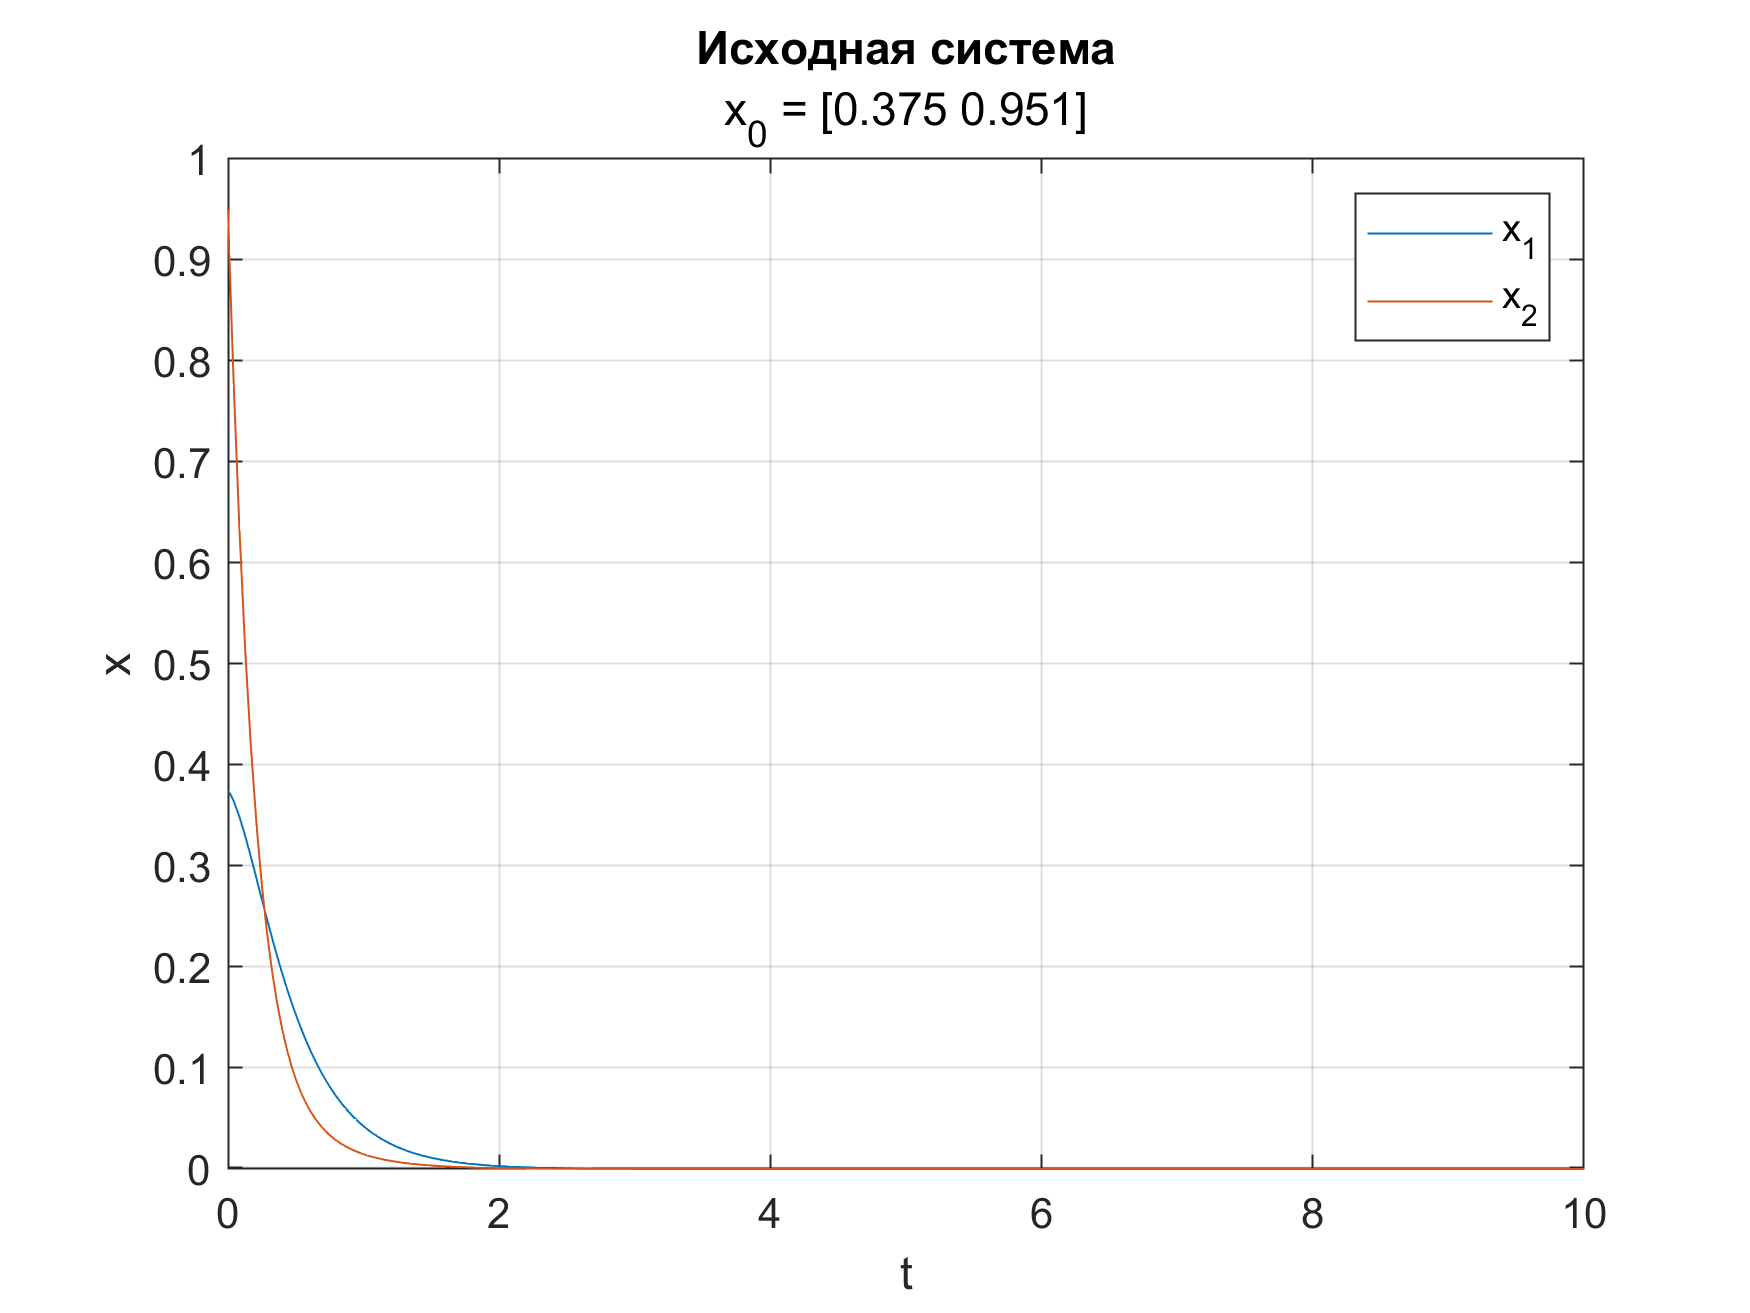
\includegraphics[width=0.7\textwidth]{initial.png}
        \caption{}
    \end{figure}

    \begin{figure}[H]
        \centering
        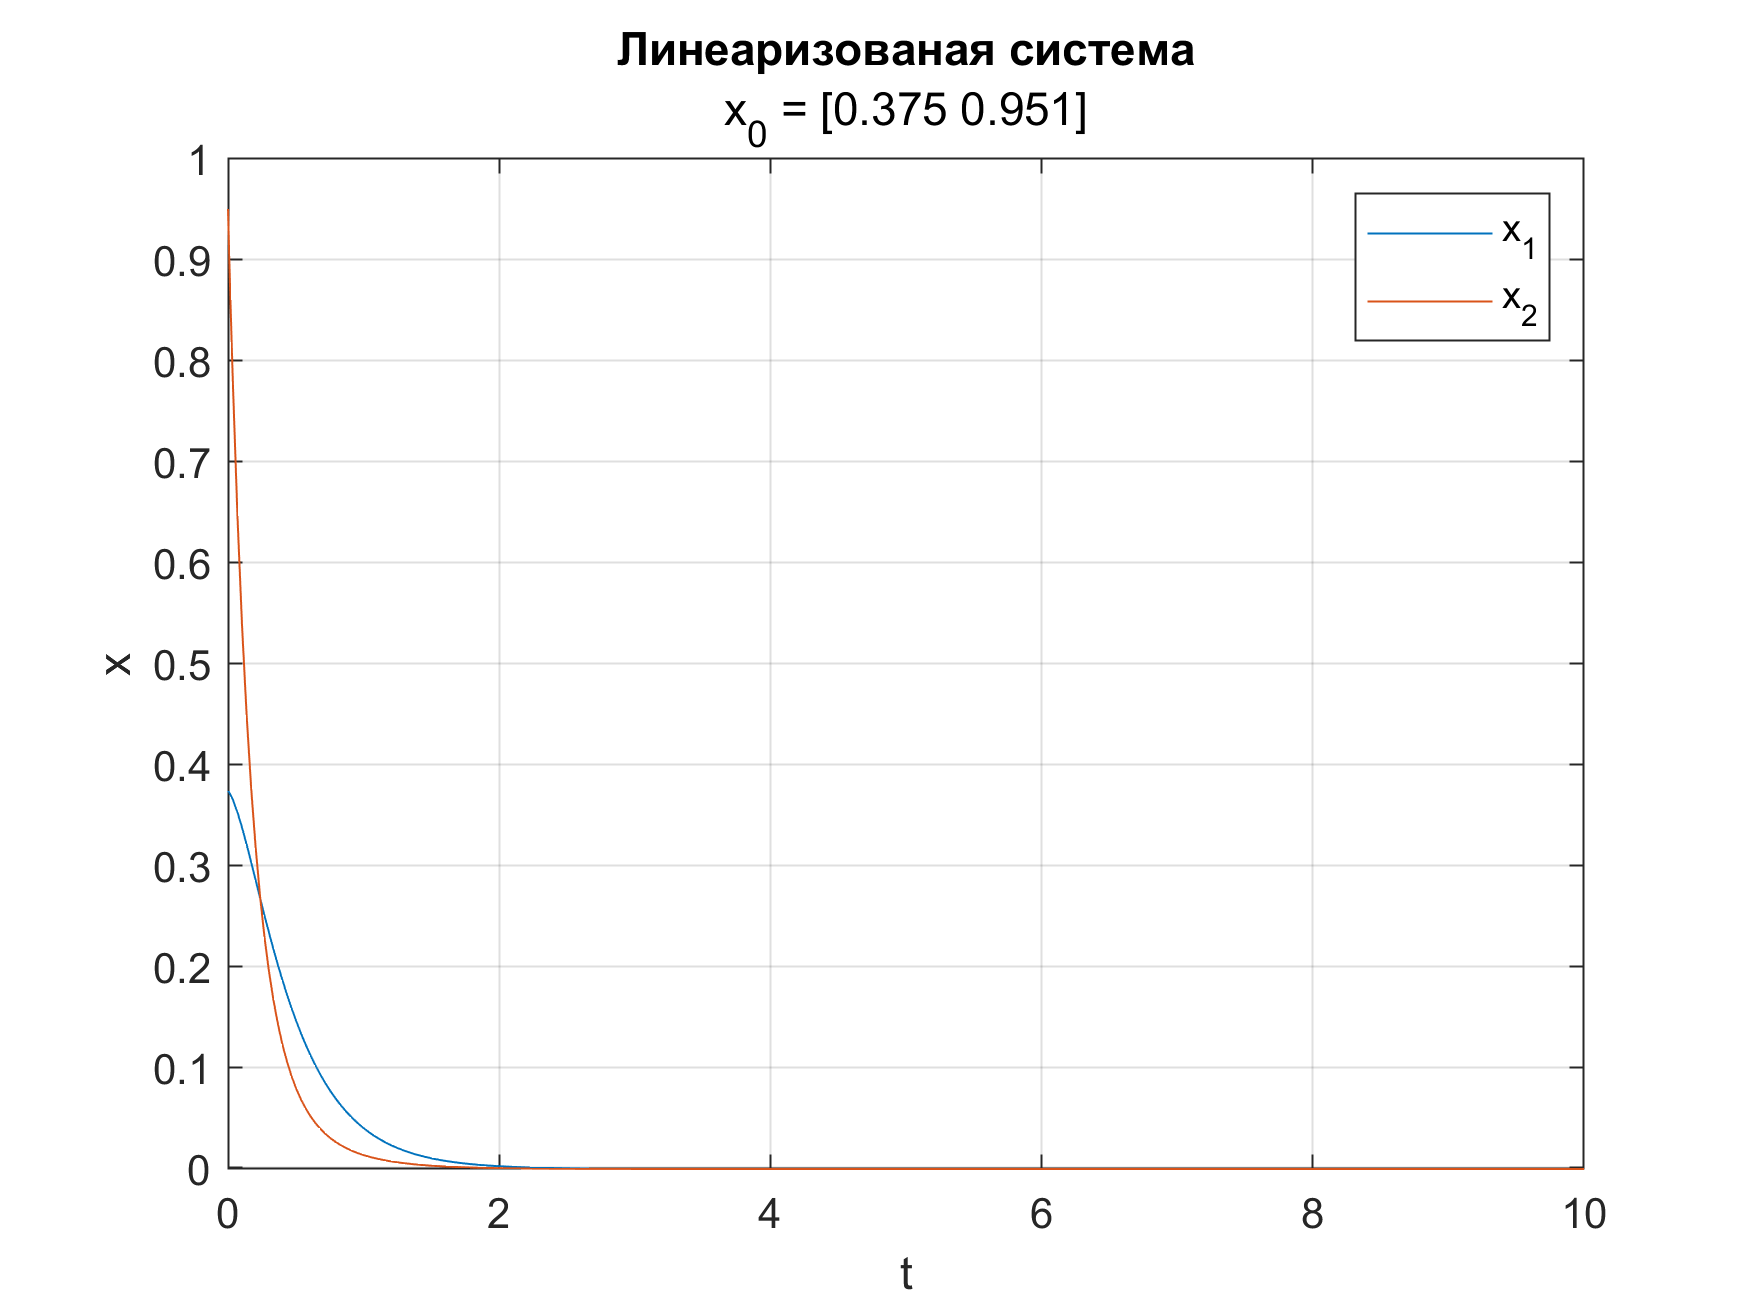
\includegraphics[width=0.7\textwidth]{linearized.png}
        \caption{}
    \end{figure}

    \section*{Задание 2}
    Дана нелинейная система
    \begin{equation*}
        \left\{
        \begin{aligned}
            \dot{x} &= Ax + b\xi,& \sigma = c^*x\\
            \xi &= \varphi(\sigma, t)=\dfrac{e^{\sigma} - e^{-\sigma}}{e^{\sigma} + e^{-\sigma}}&
        \end{aligned}
        \right.
    \end{equation*}
    \begin{equation*}
        A =
        \begin{bmatrix}
            -2& 1\\
            1& -2
        \end{bmatrix}
        , b =
        \begin{bmatrix}
            1\\
            0
        \end{bmatrix}
        , c =
        \begin{bmatrix}
            1\\
            0
        \end{bmatrix}
    \end{equation*}

    С помощью кругового критерия доказать экспоненциальную устойчивость системы.

    \subsection*{Решение}
    \subsubsection*{Проверим выполнение секторного условия}
    \begin{figure}[H]
        \centering
        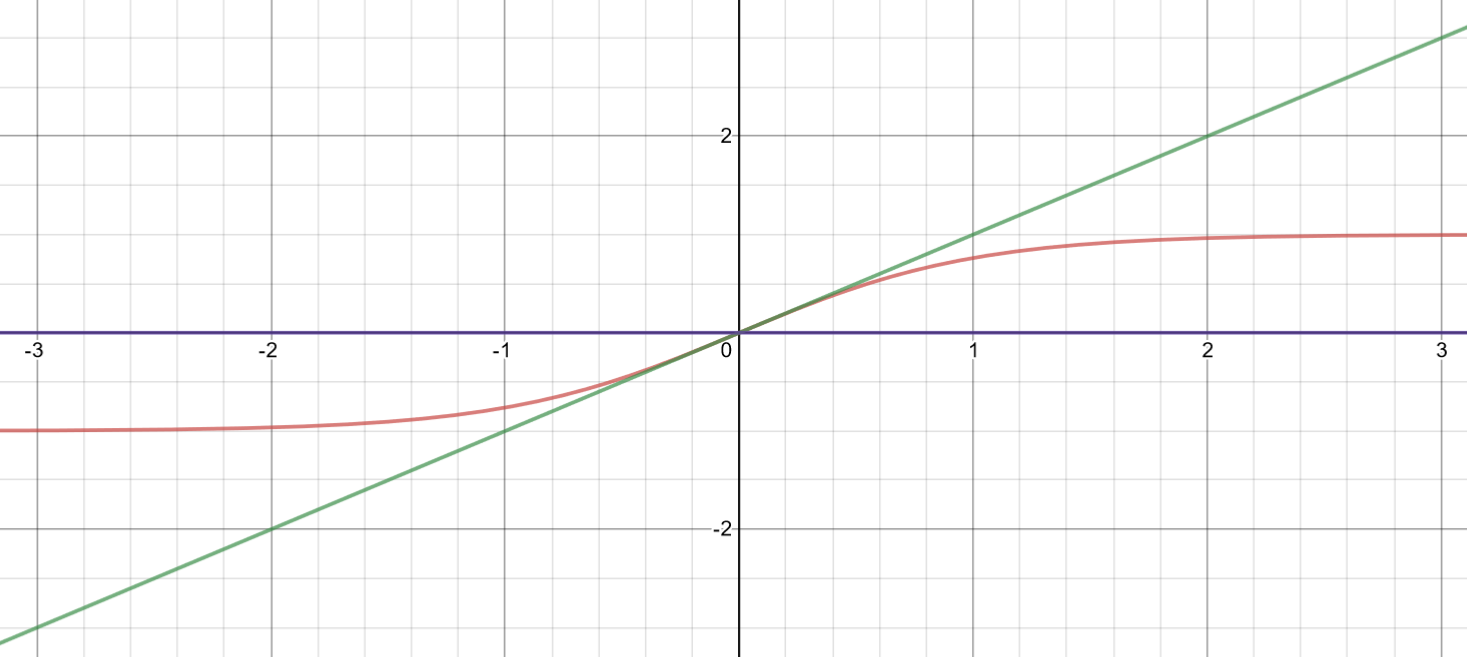
\includegraphics[width=0.7\textwidth]{phi_sector.png}
        \caption{$\varphi(\sigma, t)$, ограниченная сектором}
    \end{figure}

    \[\mu_1 \leq \dfrac{\varphi(\sigma, t)}{\sigma} \leq \mu_2 \]
    \[\mu_1\sigma \leq \dfrac{e^{\sigma} - e^{-\sigma}}{e^{\sigma} + e^{-\sigma}} \leq \mu_2\sigma \]
    \[\mu_1 \leq \dfrac{4}{(e^{\sigma} + e^{-\sigma})^2} \leq \mu_2 \]
    \[\mu_1 = 0,\,\mu_2 = 1\]

    \subsubsection*{Проверим собственные значения матрицы}
    Собственные числа матрицы $A$
    \begin{equation*}
        \begin{aligned}
            \lambda_1 &= -3 \\
            \lambda_2 &= -1
        \end{aligned}
    \end{equation*}

    Матрица не имеет чисто мнимых собственных значений.

    \subsubsection*{Проверим ассимптотическую устойчивость системы}
    Выберем $\mu_0 = \mu_1 = 0$. Тогда исследуемая система примет вид $\dot{x}=Ax$. Так как собственные числа матрицы
    известны и $Re(\lambda) < 0$, то матрица является гурвицевой, а следовательно система ассимптотически устойчива.

    \subsubsection*{Проверим <<частотное условие>>}
    \[W_0(s) = -c^*(sI - A)^{-1}b = \dfrac{-1}{s^2 + 4s + 3}\]
    \[Re\left\{ \left[ 1 + \mu_1 W_0(i\omega) \right] \left[ 1 + \mu_2 W_0(i\omega) \right]^* \right\} > 0, \,
    \omega \in \left[ -\infty,\, +\infty \right]\]
    \[\dfrac{\omega^4 + 11\omega^2 + 6}{\omega^4 + 10\omega^2 +9} > 0\]

    Условие выполняется, следовательно система экспоненциально устойчива.

    \section*{Задание 3}
    Дана нелинейная система
    \begin{equation*}
        \left\{
        \begin{aligned}
            \dot{x} &= Ax + b\xi,& \sigma = c^*x\\
            \xi &= \varphi(\sigma)=\left\{
            \begin{aligned}
                &2\sigma, &\mbox{при}\,\left| \sigma \right| < 1\\
                &2sign\sigma, &\mbox{при}\,\left| \sigma \right| \geq 1
            \end{aligned}\right.&
        \end{aligned}
        \right.
    \end{equation*}
    \begin{equation*}
        A =
        \begin{bmatrix}
            -1& -3\\
            -1& -4
        \end{bmatrix}
        , b =
        \begin{bmatrix}
            1\\
            0
        \end{bmatrix}
        , c =
        \begin{bmatrix}
            0\\
            1
        \end{bmatrix}
    \end{equation*}

    С помощью критерия Попова доказать асимптотическую устойчивость системы.

    \subsection*{Решение}

    \subsubsection*{Проверим выполнение секторного условия}
    \begin{figure}[H]
        \centering
        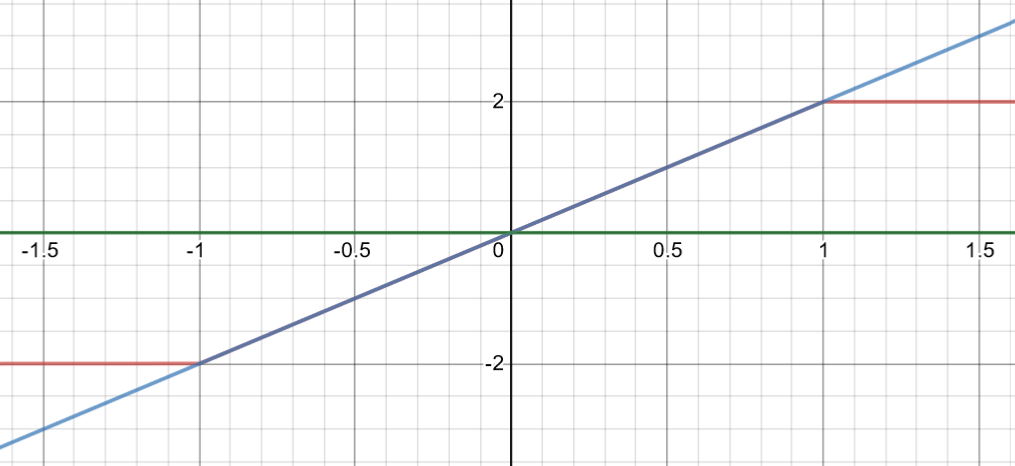
\includegraphics[width=0.7\textwidth]{phi_sector_2.png}
        \caption{$\varphi(\sigma)$, ограниченная сектором}
    \end{figure}
    \[0 \leq \dfrac{\varphi(\sigma)}{\sigma} \leq \mu_2 \leq +\infty\]
    \begin{equation*}
        0 \leq
        \left\{
        \begin{aligned}
            &2, &\mbox{при}\,\left| \sigma \right| < 1\\
            &0, &\mbox{при}\,\left| \sigma \right| \geq 1
        \end{aligned}
        \right.
        \leq \mu_0
    \end{equation*}
    \[\mu_2 = 2\]

    \subsubsection*{Проверим является матрица $A$ гурвицевой}
    Собственные числа матрицы $A$
    \begin{equation*}
        \begin{aligned}
            \lambda_1 &= -3 \\
            \lambda_2 &= -1
        \end{aligned}
    \end{equation*}
    Числа действительные и отрицательные, следовательно матрица гурвицева

    \subsubsection*{Проверим частотное условие}
    \[W_0(s) = -c^*(sI - A)^{-1}b = \dfrac{-1}{s^2 + 4s + 3}\]
    \[\mu_0^{-1} + Re\left[ \left( 1 + i\omega\nu \right) W_0(i\omega) \right] > 0, \,
    \omega \in \left[ 0,\, +\infty \right]\]
    \[\dfrac{\omega^4 + \omega^2(10\nu +21) + 3}{(\omega^2 + 1)^2 +25\omega^2} > 0 \]
    Выбрав $\nu \geq 0$ условие выполняется, следовательно система асимптотически устойчива.


    \section*{Вывод}
    В работе изучены методы исследования системы на устойчивость, а также теоремы для доказательства различных типов устойчивости -
    круговой критерий, критерий Попова и метод функций Ляпунова.

\end{document}
